% Template for Cogsci submission with R Markdown

% Stuff changed from original Markdown PLOS Template
\documentclass[10pt, letterpaper]{article}

\usepackage{cogsci}
\usepackage{pslatex}
\usepackage{float}
\usepackage{caption}

% amsmath package, useful for mathematical formulas
\usepackage{amsmath}

% amssymb package, useful for mathematical symbols
\usepackage{amssymb}

% hyperref package, useful for hyperlinks
\usepackage{hyperref}

% graphicx package, useful for including eps and pdf graphics
% include graphics with the command \includegraphics
\usepackage{graphicx}

% Sweave(-like)
\usepackage{fancyvrb}
\DefineVerbatimEnvironment{Sinput}{Verbatim}{fontshape=sl}
\DefineVerbatimEnvironment{Soutput}{Verbatim}{}
\DefineVerbatimEnvironment{Scode}{Verbatim}{fontshape=sl}
\newenvironment{Schunk}{}{}
\DefineVerbatimEnvironment{Code}{Verbatim}{}
\DefineVerbatimEnvironment{CodeInput}{Verbatim}{fontshape=sl}
\DefineVerbatimEnvironment{CodeOutput}{Verbatim}{}
\newenvironment{CodeChunk}{}{}

% cite package, to clean up citations in the main text. Do not remove.
\usepackage{cite}

\usepackage{color}

% Use doublespacing - comment out for single spacing
%\usepackage{setspace}
%\doublespacing


% % Text layout
% \topmargin 0.0cm
% \oddsidemargin 0.5cm
% \evensidemargin 0.5cm
% \textwidth 16cm
% \textheight 21cm

\title{Rapid Acquisition of Disjunction from Prosody and Consistency}


\author{{\large \bf Masoud Jasbi} \\ \texttt{masoudj@stanford.edu} \\ Department of Linguistics \\ Stanford University \And {\large \bf Akshay Jaggi} \\ \texttt{ajaggi@stanford.edu} \\ Department of Linguistics \\ Stanford University \And {\large \bf Michael C. Frank} \\ \texttt{mcfrank@stanford.edu} \\ Department of Psychology \\ Stanford University }

\begin{document}

\maketitle

\begin{abstract}
Ambiguity poses a challenge to children learning the meaning of words.
For example, a disjunction such as \texttt{A\ or\ B} can be interpreted
as inclusive (A or B, or both) or exclusive (A or B, not both).
Linguistic studies suggest that the core meaning of \emph{or} is
inclusive and despite the dominance of exclusive interpretations,
children successfully and quickly learn the meaning of \emph{or} as
inclusive. This raises a larning puzzle: how can children quickly learn
what they rarely hear? We argue that children can use the regularities
of \emph{or} in child-directed speech to learn the interpretation of a
disjunction from a few examples.

\textbf{Keywords:}
language acquisition; word learning; logical words; and; or; nativism;
constructivism.
\end{abstract}

\section{Introduction}\label{introduction}

The social media company LADbible reported the following in a tweet:
``James Bond producer says next 007 could be black \textbf{or} a
woman''. A twitter user named Robert responded sarcastically with: ``if
only women could be black!'' What in the producer's speech gave the
impression that the next 007 could not be both black \textbf{and} a
woman? The word \emph{or}. A disjunction like ``A or B'' is associated
with two interpretations: \textbf{inclusive}, and \textbf{exclusive}.
``A or B'' is inclusive when it is interpreted as ``A or B \textbf{or
both}''. This is probably what LADbible meant when reporting the James
Bond producer. However, ``A or B'' can also be exclusive: ``A or B, but
\textbf{not both}''. Robert's response shows that he had an exclusive
interpration of \emph{or}. What factors determine the interpretation of
\emph{or} and how do children learn its meaning given this ambiguity?

A large body of research in linguistics and philosophy in the past 50
years has created a common consensus on the meaning of \emph{or} (see
Aloni (2016)). Data on the interpretation of disjunction across
different sentences, contexts, and even languages show that the core
meaning of disjunction words such as \emph{or} is \textbf{inclusive}.
This is similar to the definition of disjunction in formal logics. The
\textbf{exclusive} interpretation of \emph{or} is the result of
enhancing its inclusive semantics via other (extra-semantic) factors
such as intonation (Pruitt \& Roelofsen, 2013), inconsistency of the
options (Geurts, 2006), and pragmatic reasoning over the speaker's
choice of \emph{or} instead of \emph{and} (Grice, 1975). Therefore,
interpreting a disjunciton is a complex process that needs to take into
account the meaning of \emph{or} as well as different structural and
contextual factors that accompany it. How do we, as children, learn such
a complex interpretive system?

There are two accounts of children's acquisition of disjunciton: a
\textbf{constructivist} account, and 2. a \textbf{nativist} account.
Under the constructivist account, children learn the meaning of
\emph{or} by paying attention to how parents use it in different
contexts. They form usage-rules and expand their usage repertoire as
they grow up. The prediction is that children's production of \emph{or}
is slow and gradual, mirroring what they hear from parents. Morris
(2008) found that \emph{and} is about 13 times more frequent than
\emph{or} in parents' speech to children. As predicted by the
constructivist account, Morris (2008) reported that children also learn
to produce \emph{and} much more quickly than \emph{or}. They reach the
adult rate of \emph{and} at age 3 while for \emph{or} there is a gradual
increase in production, possibly reaching the adult level at ages 5 or
6. The faster acquisition of \emph{and} is consistent with the
constructivist theory that emphasizes the role of usage frequency in
children's linguistic development. Morris (2008) also reported that the
majority of \emph{or} examples children hear are exclusive. He argued
that consistent with the constructivist account, the majority of
\emph{or}'s children produce are also exclusive. Therefore, the
inclusive semantics of \emph{or} is developed after the exclusive
interpretation.

However, several comprehension studies of \emph{or} in different
linguistic contexts show that children as young as three-years old
interpret \emph{or} as inclusive disjunction (Crain, 2012). This is
surprising given Morris (2008)`s finding that the majority of \emph{or}
examples children hear are exclusive. How do children learn the
interpretation of disjunction as inclusive if they rarely hear it? We
call this the \textbf{learning puzzle of disjunction}. Crain (2012)
suggests that instead of learning from the parents' usage of \emph{or},
children rely on the innate knowledge that the the disjunciton operator
in their native language must have an inclusive meaning. This nativist
account predicts that \emph{or} is learned relatively quickly and
accurately by children.

Here we present an alternative answer that provides a synthesis between
the nativist and constructivist accounts. We show that children can use
regularities in parents' usage of \emph{or} to learn the interpretation
of disjunction from a handful of examples. In study 1, we use a large
scale corpus study of parents and children's speech to show that both
\emph{and} and \emph{or} appear relatively quickly in children's speech
and reach the adult rate by the age 4. This finding is consistent with
the comprehension studies that show children have an adult-like
understanding of these words by the age four. In study 2, we replicate
Morris (2008)'s finding that the majority of \emph{or} examples in
child-directed speech have an exclusive interpretation. However, we also
show that these exclusive interpretations correlate systematically with
two factors external to \emph{or}: intonation and consistency of the
options. Exclusive interpretations are either inconsistent in nature
(e.g.~clean or dirty) or carry a distinct rise-fall intonation. We show
that setting aside these cases, the interpretation of a disjunction is
inclusive.

We argue that if children track the interpretive cues that accompany a
disjunction, they can tease apart the role of the word \emph{or} from
factors that accompany and enhance it to shape the exclusive
interpretation. This way children can discover that exclusivity
corrleates with rise-fall intonation and inconsistent options, while
\emph{or} itself does not exclude the option of both disjuncts being
true. We implement this novel account in a decision-tree that correctly
learns to predict the interpretation of a disjunction with 80\% accuracy
after only a few examples. Our results show that the richness and
systematicity of children's linguistic input allows rapid acquisition of
disjunction with no need for an innate assumptions specific to the
meaning of disjunction. We discuss the important implications of this
work for the theories of word learning in the last section.

\section{Study 1: Corpus Study}\label{study-1-corpus-study}

First, we conducted an exploratory and large scale investigation of
\emph{and} and \emph{or} productions in parents and children. The goal
of the study was to find out when children start producing these words
and when they reach the adult rate of production. We conclude that
children start producing \emph{and} around 1.5 or 2 years of age, and
\emph{or} between the ages of 2 and 3. They reach the adult rate of
production for \emph{and} around 3 and for \emph{or} around 4 or
possibly earlier.

\subsection{Methods}\label{methods}

We accessed the Child Language Data Exchange System (CHILDES, MacWhinney
(2000)) via the online platform
\href{http://childes-db.stanford.edu/}{childes-db} and its associated R
package childesr (Sanchez et al., in prep). We extracted all instances
of \emph{and} and \emph{or} from the English corpora (ENG-NA and
ENG-UK). We limited our analysis to the data between one and six years
because there is scarce data outside this age range. We computated the
relative frequency of connective production by dividing the total number
of \emph{and}/\emph{or} in the speech of fathers, mothers, and children
at a particular age by the total number of words spoken at that age. We
present the relative frequency as parts per thousand.

\subsection{Results}\label{results}

In figure 1, we show the relative frequencies of \emph{and} and
\emph{or} in the speech of parents and children between one and six
years. It is important to note that the y-axes for \emph{and} vs.
\emph{or} show different ranges. This is due to the big difference in
the relative frequencies of \emph{and} and \emph{or}. In the speech of
parents, \emph{and} is produced around 20 times per thousand words while
\emph{or} is only produced around 2 times per thousand words. This
confirms previous findings that \emph{or} is much less frequent in child
directed speech than a similar funciton word such as \emph{and}.

\begin{CodeChunk}
\begin{figure}[H]
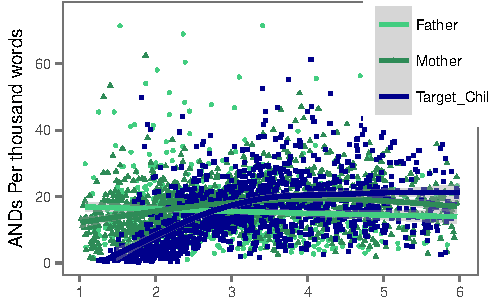
\includegraphics{figs/OverallConnectivePlots-1} 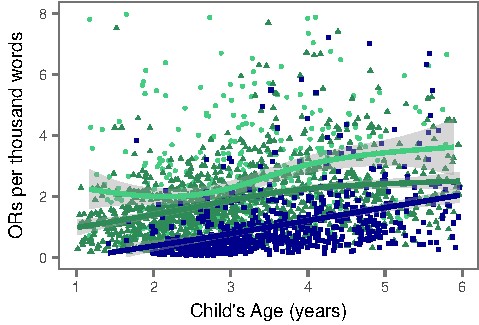
\includegraphics{figs/OverallConnectivePlots-2} \caption[The relative frequency of AND (top) and OR (bottom) per thousand words in the speech of fathers, mothers, and children between the ages of 1 and 6]{The relative frequency of AND (top) and OR (bottom) per thousand words in the speech of fathers, mothers, and children between the ages of 1 and 6.}\label{fig:OverallConnectivePlots}
\end{figure}
\end{CodeChunk}

\emph{And} and \emph{or} seem to show different developmental
trajectories in the speech of children. For \emph{and}, there is a rapid
increase in its production between the ages of 1.5 and 3 before it
reaches the adult rate around the age 3 and stay at that level until the
age 6. For \emph{or}, on the other hand, we see a slow incrase from the
age 2 until the age 6 when it reaches the adult rate. This difference in
the development of \emph{and} \& \emph{or} production was attributed to
the frequency of these items in child-directed speech. Since \emph{and}
is much more frequent than \emph{or}, it is learned much faster than
\emph{or}. Morris (2008) argued that such patterns support the
item-based and usage-based acquisition of logical words.

However, the analysis above does not control for other factors that can
affect the production of words by children. An important factor to
control for is the development of speech acts. While content words such
as \emph{dog} or \emph{chair} may appear freely in different types of
speech acts, function words are highly constrained by the type of speech
acts they can appear in. For example, it is reasoable to assume that
question words such as \emph{how} and \emph{why} are much more likey to
occur in questions than statements (declaratives). If parent-child
interaction is such that parents ask more questions than children, it is
not surprising to find higher rates of \emph{how} and \emph{why}
production in parents than children. Therefore, it is important to
control for the speech act a function word appears in.

Figure 2 shows the relative frequencies of \emph{and} and \emph{or} in
questions vs.~declaratives, in the speech of parents and children
between one and six years. Here, the relative frequency is computed by
dividing the total number of \emph{and}/\emph{or} in a
question/declarative in the speech of fathers, mothers, and children at
a particular age, by the total number of words in a question/declarative
spoken at that age. As before, we present the relative frequency as
parts per thousand.

\begin{CodeChunk}
\begin{figure}[H]
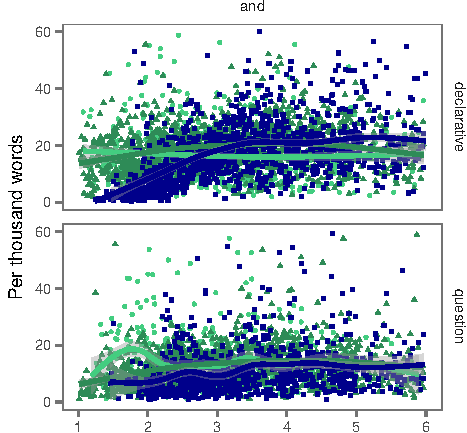
\includegraphics{figs/byspeechActPlots-1} 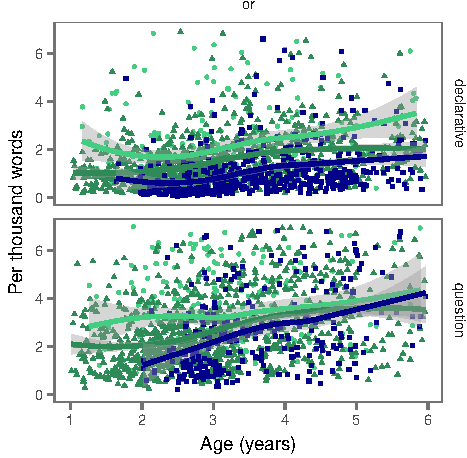
\includegraphics{figs/byspeechActPlots-2} \caption[The relative frequency of AND (top) and OR (bottom) per thousand words in delcaratives and questions in the speech of fathers, mothers, and children between the ages of 1 and 6,]{The relative frequency of AND (top) and OR (bottom) per thousand words in delcaratives and questions in the speech of fathers, mothers, and children between the ages of 1 and 6,}\label{fig:byspeechActPlots}
\end{figure}
\end{CodeChunk}

The results show similar developmental trajectories for the production
of \emph{and} and \emph{or} in children. For both words, there is a
relatively rapid incease in their frequency between the ages of 2 and 4
before reaching the parent rate at the age of 4 and staying at that rate
until the age of 6. This pattern of production is consistent with the
nativist observations that the acquisition of \emph{and} and \emph{or}
is rapid and that children have an adult-like comprehension of these two
connectives at the age 4.

\subsection{Summary}\label{summary}

And is a lot more frequent than or in child directed speech.

In the first six years, it appears that children reach the adult
production rate for and but not or.

This is at least partly because or is more frequent in questions and
children produce fewer questions than parents.

The developmental trajectory of connective production is best described
as a quick increase in production between the ages of 2 and 4 and
staying around the parents' rate between the ages 4 and 6. This is
compatible with the comprehension studies which suggest children
understand \emph{and} and \emph{or} by the age four.

\section{Study 2: Annotation Study}\label{study-2-annotation-study}

Second, we conducted an detailed and small-scale investigation of
\emph{or} productions in parents and children. The goal of the study was
to find out how children learn the meaning of \emph{or} from such little
data. We conclude that children hear significantly more exclusive
\emph{or} supporting Morris (2008)'s findings. Additionally, we find
that the exclusive uses of \emph{or} are rich in structures that index
the exclusive interpretation. These indicative structures include
specifically intonation and consistency of the disjuncts. Exclusive
interpretations are either inconsistent in nature (e.g.~clean or dirty)
or carry a distinct rise-fall intonation. We then show that a decision
tree model can learn to accurately (\textgreater{}80\%) predict
exclusivity using this information after seeing few (\textless{}20)
examples.

\subsection{Methods}\label{methods-1}

We accessed the Providence corpus via CHILDES (Demuth, Culbertson, \&
Alter, 2006). We extracted all instances of \emph{or} along with the two
utterances before and after the utterance containing \emph{or}. We
annotated the examples for four major categories. \emph{Exclusivity
Interpretation}: This category represents the goal task: understanding
the intended form of disjunction. \emph{Intonation}: This category was
divided into three main intonation patterns over the disjuncts.
Intonation could be flat, rising overall, or rise-fall. These three
categories were selected because rise-fall in particular has been shown
to lead to an exclusive interpretation of the disjunction
({\textbf{???}}). \emph{Consistency}: This category tracked the logical
consistency of the disjuncts. Two disjuncts were marked as inconsistent
if replacing the word ``or'' with ``and'' produced a logical conflict.
For example in ``Are your feet clean or dirty?'', the disjuncts are
inconsistent: the addresee's feet cannot be both clean and dirty.

Two raters annotated the same 240 utterances to develop a reliability
score. The interrater reliability was calculated over 8 iterations of 30
examples. Training only completed after 3 consecutive iterations with
reliability over 0.7 for all categories.

\subsection{Results}\label{results-1}

First, similar to Morris (2008), we found that the majority of \emph{or}
examples in CDS receive an exclusive interpretation (\(\sim\)\%65).
Figure 3 shows this difference in distribution. However, the rate of
exclusive interpretations change systematically when we break the data
down by prosody and consistency (figure below). A mixed-effects binomial
logistic regression with the fixed effects of intonation, consistency,
and random effects for children found intonation and consistency
significant in interpreting disjunctions. Disjunctions were more likely
to be interpreted as exlclusive if they received a rise-fall intonation
(\(\beta\)=-3.79, \(z\)=1.66, \(p < 0.001\)) or if they were
inconsistent(\(\beta\)=-2.2, \(z\)=2.08, \(p < 0.001\)). Disjunctions
were more likely to be interpreted as inclusive if they were consistent
and received a rising intonation (\(\beta\)=0.58, \(z\)=0.24,
\(p < 0.001\)) or flat intonation (\(\beta\)=0.38, \(z\)=0.27,
\(p < 0.001\)).

\begin{CodeChunk}
\begin{figure}[tb]

{\centering 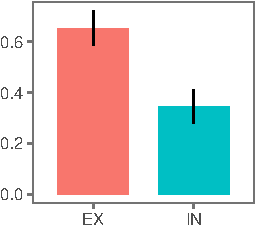
\includegraphics{figs/interpretation-1} 

}

\caption[Distribution of exclusive and inclusive interpretations broken down by intonation and consistency]{Distribution of exclusive and inclusive interpretations broken down by intonation and consistency. Error bars represent bootstrapped 95\% confidence intervals}\label{fig:interpretation}
\end{figure}
\end{CodeChunk}

Figure 4 demonstrates the clear relationship between exclusive
interpretation, rise-fall intonation, and inconsistent disjuncts.
Without these markers of exclusivity, the inclusive interpretations
remain. This supports Crain (2012)'s claim that the ``default''
interpretation of ``or'' is inclusive.

\begin{CodeChunk}
\begin{figure*}[h]

{\centering 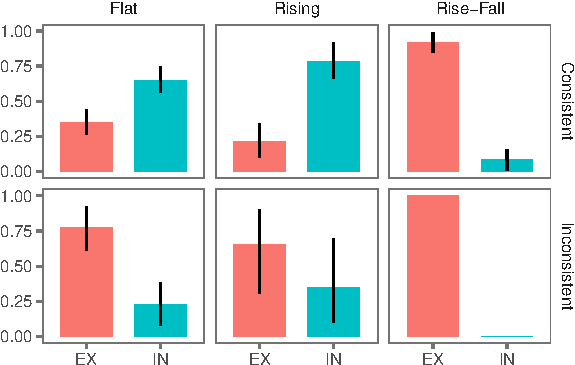
\includegraphics{figs/interpretationByIntonationAndConsistency-1} 

}

\caption[Distribution of exclusive and inclusive interpretations broken down by intonation and consistency]{Distribution of exclusive and inclusive interpretations broken down by intonation and consistency. Error bars represent bootstrapped 95\% confidence intervals}\label{fig:interpretationByIntonationAndConsistency}
\end{figure*}
\end{CodeChunk}

Next, using Sci-kit Learn's Decision Tree Module (Pedregosa et al.,
2011), we built a predictive model to train on annotated \emph{or}
utterances and predict the exclusivity of unseen \emph{or} utterances
(annotated for intonation and consistency). Averaged over 100 trials and
training on 200 examples, the average accuracy of a binary tree was
83\%. More remarkably, the tree achieved an average of 80\% accuracy
after training on only 20 examples. The success of such a simple tree
indicates that children could use a simple model to rapidly learn the
exclusive interpretation of \emph{or} from little data.

\begin{CodeChunk}
\begin{figure}[h]

{\centering 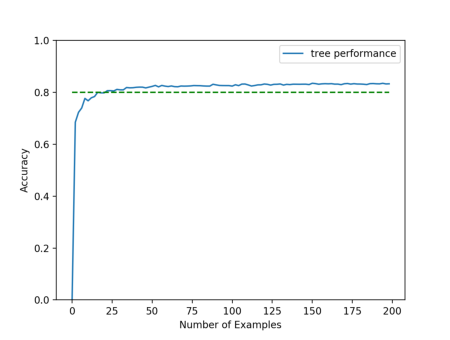
\includegraphics{figs/learningCurve-1} 

}

\caption[Decision Tree Accuracy as a function of number of examples seen]{Decision Tree Accuracy as a function of number of examples seen}\label{fig:learningCurve}
\end{figure}
\end{CodeChunk}

\subsection{Summary}\label{summary-1}

In study 2, we confirm Morris (2008)'s finding that exclusive
interpretations of \emph{or} are far more common than inclusive
interpretations. However, we also show that the majority of these
exclusive interpretations coincide with systematic indicators.
Disjunctions that are accompanied by rise-fall intonation or
inconsistent disjuncts are far more likely to be exclusive. Disjunctions
that do no bear these features are more likely to be inclusive.
Accounting for these external factors, a simple decision tree can
rapidly learn to predict the exclusive interpretation of the
disjunction.

\section{Conclusion}\label{conclusion}

List what you showed and argued for.

Talk about important implications for theories of word learning.

Possibly talk about the original tweet and how that falls still outside
what your algorithm learns.

\section{Acknowledgements}\label{acknowledgements}

Place acknowledgments (including funding information) in a section at
the end of the paper.

\section{References}\label{references}

\setlength{\parindent}{-0.1in} \setlength{\leftskip}{0.125in} \noindent

\hypertarget{refs}{}
\hypertarget{ref-Aloni2016}{}
Aloni, M. (2016). Disjunction. In E. N. Zalta (Ed.), \emph{The stanford
encyclopedia of philosophy}. Stanford University. Retrieved from
\url{https://plato.stanford.edu/archives/win2016/entries/disjunction/}

\hypertarget{ref-crain2012emergence}{}
Crain, S. (2012). \emph{The emergence of meaning}. Cambridge University
Press.

\hypertarget{ref-demuth2006word}{}
Demuth, K., Culbertson, J., \& Alter, J. (2006). Word-minimality,
epenthesis and coda licensing in the early acquisition of english.
\emph{Language and Speech}, \emph{49}(2), 137--173.

\hypertarget{ref-geurts2006exclusive}{}
Geurts, B. (2006). Exclusive disjunction without implicatures.
\emph{Ms., University of Nijmegen}.

\hypertarget{ref-grice1975logicconvo}{}
Grice, H. P. (1975). Logic and conversation. In P. Cole \& J. Morgan
(Eds.), \emph{Syntax and semantics} (Vol. 3: Speech Acts, pp. 43--58).
Academic Press.

\hypertarget{ref-macwhinney2000childes}{}
MacWhinney, B. (2000). \emph{The childes project: The database} (Vol.
2). Psychology Press.

\hypertarget{ref-morris2008logically}{}
Morris, B. J. (2008). Logically speaking: Evidence for item-based
acquisition of the connectives and \&amp; or. \emph{Journal of Cognition
and Development}, \emph{9}(1), 67--88.

\hypertarget{ref-pedregosa2011scikit}{}
Pedregosa, F., Varoquaux, G., Gramfort, A., Michel, V., Thirion, B.,
Grisel, O., \ldots{} others. (2011). Scikit-learn: Machine learning in
python. \emph{Journal of Machine Learning Research}, \emph{12}(Oct),
2825--2830.

\hypertarget{ref-pruitt2013interpretation}{}
Pruitt, K., \& Roelofsen, F. (2013). The interpretation of prosody in
disjunctive questions. \emph{Linguistic Inquiry}, \emph{44}(4),
632--650.

\hypertarget{ref-childesdb}{}
Sanchez, A., Meylan, S., Braginsky, M., MacDonald, K., Yurovsky, D., \&
Frank, M. C. (in prep). Childes-db: A flexible and reproducible
interface to the child language data exchange system (childes).

\end{document}
